\documentclass{article}
\usepackage{amsmath}
\usepackage{graphicx}
\usepackage[a4paper, margin=1in]{geometry}
\usepackage{pgfplots}
\pgfplotsset{compat=1.17}
\usepackage{afterpage}
\usepackage{float}
\usepackage{hyperref}
\usepackage{subcaption}
\graphicspath{{assets/}}

\title{Crypto Monitor on a Real Time Embedded System}
\author{Epameinondas Bakoulas}
\date{July 2025}

\begin{document}

\maketitle

\section{Objective}
Our goal in this project is to implement a crypto monitor that will run on a raspberry-pi continuously.
It will collect data via a websocket for a total of 8 different symbols, perform some calculations for
each symbol and save the results on .txt files.

Later on, we will expand on this idea by performing other calculations out of the scope of this project,
in order to better predict the market and make better decisions on when to buy or sell.

\section{Analysis}

\subsection{Overview}
Our analysis will be performed on 8 different cryptocurrency symbols, which are
BTC-USDT, ADA-USDT, ETH-USDT, DOGE-USDT, XRP-USDT, SOL-USDT, LTC-USDT, BNB-USDT, and 
we will use the the OKX Websocket public channel to collect the exchange data.

We're going to perform a total of 2 calculations for each symbol.
\begin{itemize}
    \item Calculate the moving average price and volume of the symbol for the last 15 minutes.
    \item Calculate the pearson correlation with all other symbols (and itself) using the last 8 averages (we will clarify on this later on).
\end{itemize}

These calculations are going to be performed every minute and the results will be saved on a .txt file.

\subsection{Storing measurements}
The measurements (exchanges) that arrive via the websocket will be saved in 2 places:
\begin{itemize}
    \item In-memory for quick retrieval and calculations (last 15 minutes only), on a double-ended queue.
    \item In .txt files for long-term storage and analysis, separate for each symbol.
\end{itemize}

\begin{figure}[H]
    \centering
    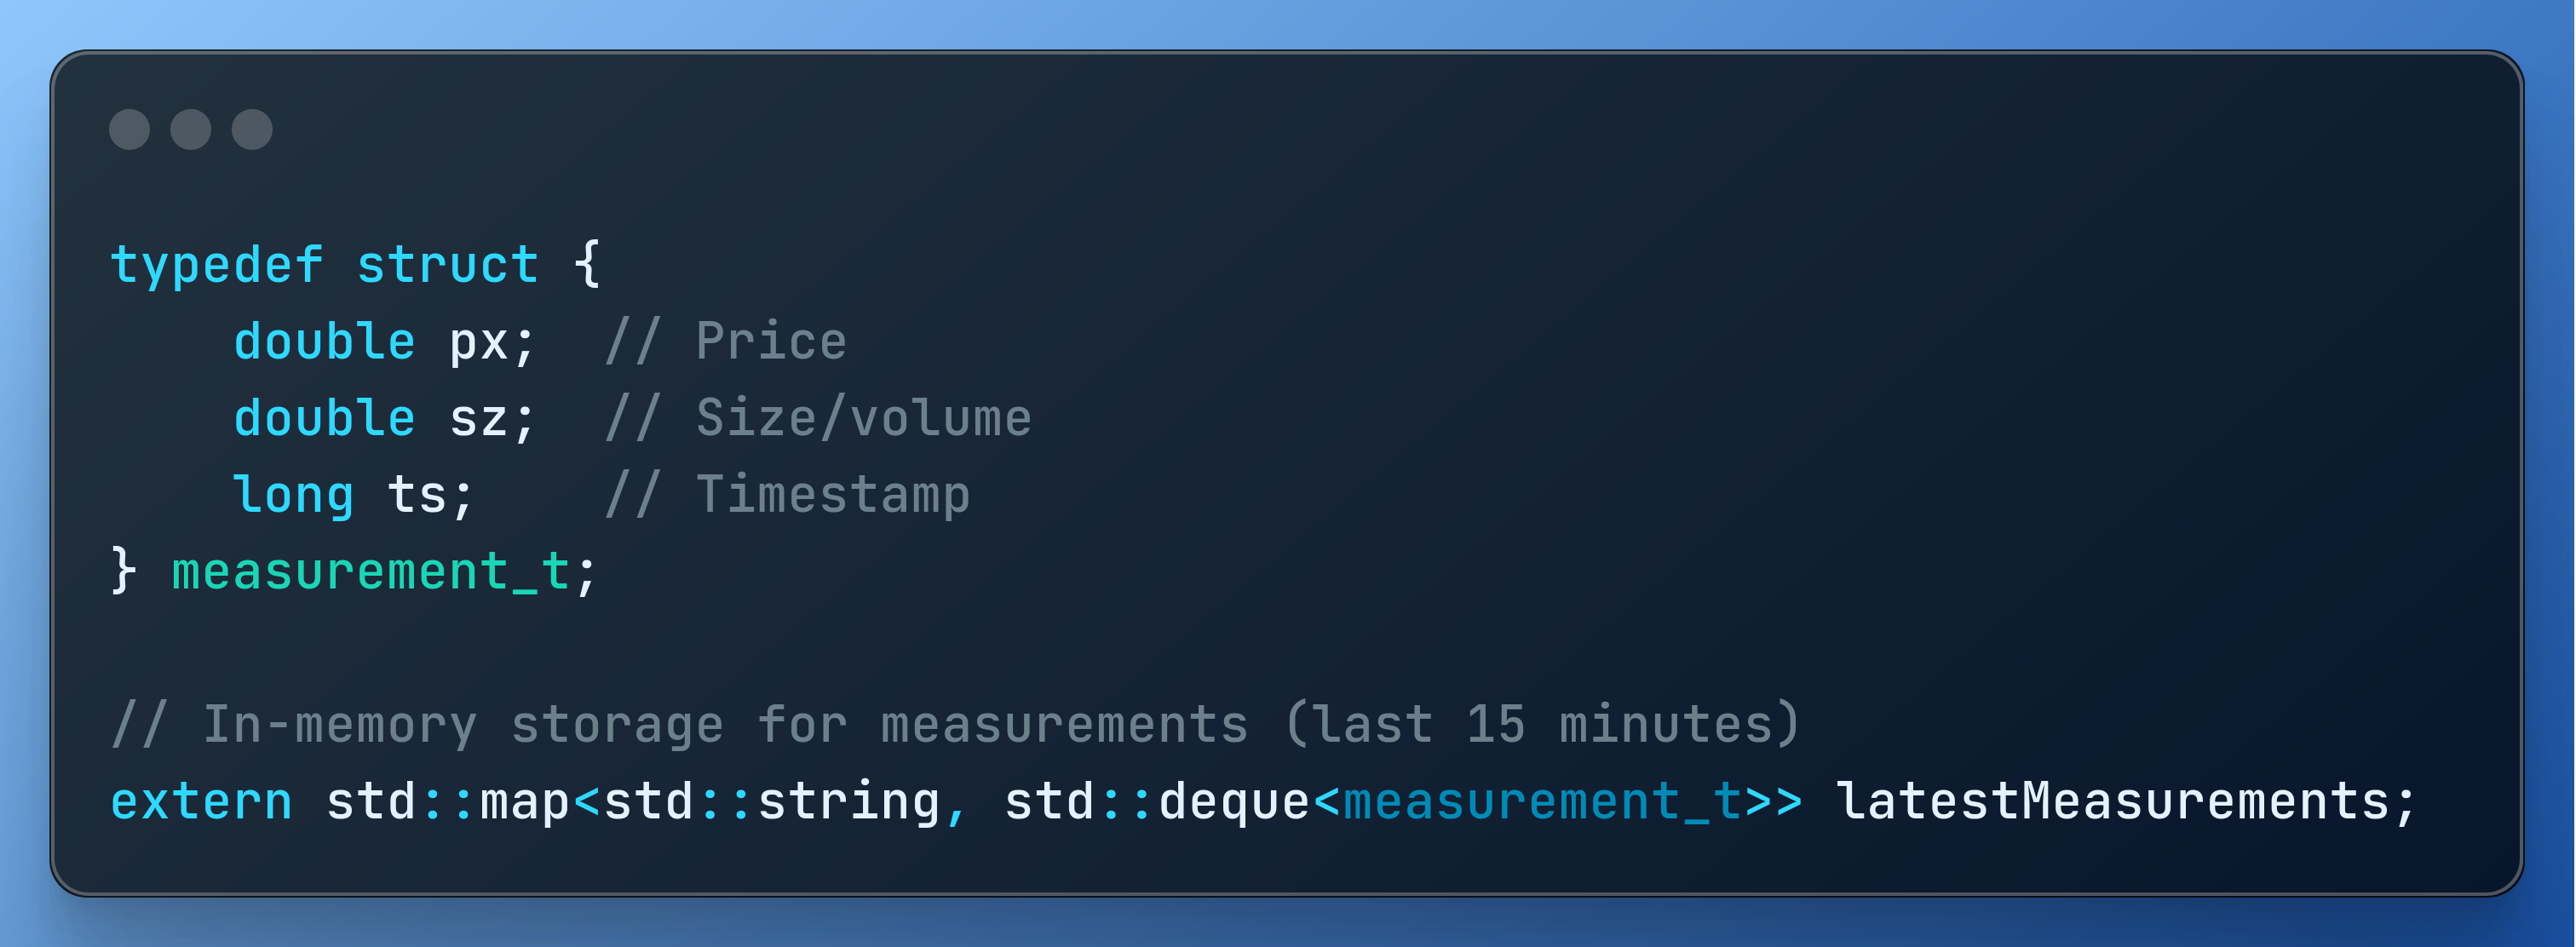
\includegraphics[width=1\textwidth]{measurement.png}
    \caption{Measurement Storage}
    \label{alg:measurements}
\end{figure}

\subsection{Scheduling}
In order to perform the calculations every minute, we will spawn a thread called \texttt{threadScheduler} that will run every minute and perform the calculations.



\section{Benchmarks}


\section{Conclusion}

The source code can be found on the \href{https://github.com/NontasBak/CUDA-bitonic-sort}{Github repository}.

\end{document}